\section{Introduction To Data Management and Data Warehouse}

%%%%%%%%%%%%%%%%%%%%%%%%%%%%%%%%%%%%%%%%%%%%%%%%%%%%%%%%%%%%%%%%%%%%%%%%%%%%%%%%%%%%%%%%%

\begin{frame}
\frametitle{Chapter Objectives}

\begin{itemize}
	\item<1-> Be familiar with data management life-cycle. \pause
	\item<2-> Introduction to data warehouse and its usage. \pause	
	\item<3-> Motivation to DWH.\pause
	\item<4-> What is the different types of DWH?\pause
	\item<5-> Use cases\pause
	\item<6-> Data Encoding and Formats\pause	
	\item<6-> Challenges to build a DWH.\pause
	\item<7-> Data modeling design.\pause
\end{itemize}

\end{frame}

%%%%%%%%%%%%%%%%%%%%%%%%%%%%%%%%%%%

\subsection{Data Management}

\begin{frame}
\frametitle{Data Management}

\begin{itemize}
\item Data are a product.
\item Data product has a life-cycle as following (simplified): 
\begin{itemize}
	\item \textbf{Question}, Idea, or service.
	\item \textbf{Identifying} the source of information and the data type ex: (text, images, videos, audio, or sensors).
	\item \textbf{Document} all details regarding the data including quality, security, efficiency, and access (consideration during the cycle).
	\item Delivery automation (Tools and Process) AKA \textbf{DevOps} cycle.
	\item \textbf{Extraction} Process (collection).
	\item \textbf{Transformation} ex: (cleansing, Apply business logic, Organize).
	\item \textbf{Loading} or store the transformed data based on our usage or use case.
	\item Business Intelligence (\textbf{BI}) or data discovery (continues process).
	\item \textbf{Integration} and publishing.
	\item Data retention or \textbf{archiving} process ex: (Hot or Cold storage).
\end{itemize}
\end{itemize}

\end{frame}

%%%%%%%%%%%%%%%%%%%%%%%%%%%%%%%%%%%%%%%%%%%%%%%%%%%%%%%%%%%%%%%%%%%%%%%%%%%%%%%%%%%%%%%%%

\begin{frame}
\frametitle{Data Management Life-Cycle}
\begin{center}			
\smartdiagramset{circular distance=3.5cm,
font=\scriptsize,
%				text width=1cm,
module minimum width=2cm,
circular distance =3.4cm,
module minimum height=.1cm,
arrow tip=to}
\smartdiagram[circular diagram]{Archiving,Idea, Identify, Document, 				
DevOps,Extraction, Loading, BI, Integration}


\end{center}

\end{frame}

%%%%%%%%%%%%%%%%%%%%%%%%%%%%%%%%%%%%%%%%%%%%%%%%%%%%%%


\subsection{From DWH to Big Data}
\begin{frame}
\frametitle{Motivation to Data Warehouse}
\begin{itemize}[<+->]
\item Data could be a product for some companies.
\item It could be decision support for other products or businesses.
\item Reporting the results after pass the data life-cycle will be from storage (Database).
\item There are some challenges facing the people who work on data management backend:
\begin{itemize}
\item Performance.
\item Integration.
\item Applying analytical functions. %Moving average
\end{itemize}
\item Vendors who are working to solve the above challenges creating their own product of DWH and their ultimate work is to optimize the above points.
\end{itemize}
\end{frame}

%%%%%%%%%%%%%%%%%%%%%%%%%%%%%%%%%%%%%%%%%%%%%%%%%%%%%%
\begin{frame}
\frametitle{Motivation to Data Warehouse (DWH)}
\begin{columns}[T] % align columns

\begin{column}{.58\textwidth}
\begin{itemize}
\item The DWH is not a product but an environment.
\item It is a process of transforming data into information and make it available to users in a \textbf{timely manner} to make a difference.
\item It is an architectural construct of an information system which provides users with current and historical decision support information which is difficult to access or present in the traditional operational data store.
\item The DWH is the core of the BI system which is built for data analysis and reporting.
\end{itemize}

\end{column}%
\hfill%
\begin{column}{.38\textwidth}
\begin{definition}[What is Data Warehousing?] A DWH is defined as a technique for collecting and managing data from varied sources to \textbf{provide meaningful business insights}. It is a blend of technologies and components which aids the strategic use of data.%\footnotemark
\end{definition}

\end{column}%
\end{columns}
%\footnotetext{The definition mentioned in this slides copied from  \href{https://www.guru99.com/data-warehousing.html\#2}{guru99.com} }

\end{frame}

%%%%%%%%%%%%%%%%%%%%%%%%%%%%%%%%%%%%%%%%%%%%%%%%%%%%%%
\begin{frame}
\frametitle{Motivation to Data Warehouse}

Data warehouse system is also known by the following names:


\begin{wideitemize}
\item Decision Support System (DSS).
\item Business Intelligence Solution.
\item Executive Information System.
\item Management Information System.
\item Analytic Application.
\item Data Warehouse.

\end{wideitemize}

The real concept was given by Inmon Bill. He was considered as a father of the DWH. He had written about a variety of topics for building, usage, and maintenance of the warehouse \& the Corporate Information Factory

\end{frame}

%%%%%%%%%%%%%%%%%%%%%%%%%%%%%%%%%%%%%%%%%%%%%%%%%%%%%%
\begin{frame}
\frametitle{Motivation to Data Warehouse}
Types of Data Warehouse
\begin{description}
\item [\textbf{Enterprise Data Warehouse (EDWH)}] It provides decision support service across the enterprise. It offers a unified approach for organizing and representing data (DWH Model). It offers data classifications according to the subject with privileges policy.
\item [\textbf{Operational Data Store (ODS):}] is a central database that provides an up-to-date (real-time) data from multiple transnational systems for operational reporting into a single DWH.

%% for real time questions and answers. call ODS using intermidiate data store. DWH is day -1 (billing & subscribtions). Oracle (Loading or headache) && CDC capture change interest column not row
\item [\textbf{Data Mart:}] A data mart is a subset of the data warehouse. It specially designed for a particular line of business, such as sales, finance, sales or finance. In an independent data mart, data can collect directly from sources.
\end{description}

\end{frame}

%%%%%%%%%%%%%%%%%%%%%%%%%%%%%%%%%%%%%%%%%%%%%%%%%%%%%%

%%%%%%%%%%%%%%%%%%%%%%%%%%%%%%%%%%%%%%%%%%%%%%%%%%%%%%

\begin{frame}
\frametitle{DWH vs ODS vs Data Mart}


\begin{table}[t]
\centering	
\resizebox{\columnwidth}{!}{%

%		\centering
\begin{tabular}{|c | c | c| c |}
\hline
\textbf{Metric}  & \textbf{DWH}& \textbf{ODS} & \textbf{Data Mart} \\
\hline
Latency & Day -1  & Real-time & Day -1 \\			
Data level  & Transnational & Transnational & Summary \\
Historical  & Long-term & Snapshot & Aggregated Long-Term \\
Size & TB/PB & GB & GB/TB\\
Orientation & Multi sources & Multi sources & Product\\
Business Units & Multi organizational units & Product team & Business team \\
\hline
\end{tabular}
%		\caption{Data Representation Combination Matrix}\label{Tab:Data_Representation_Matrix}
}
\end{table}
\end{frame}


%%%%%%%%%%%%%%%%%%%%%%%%%%%%%%%%%%%%%%%%%%%%%%%%%%%%%%

\begin{frame}
\frametitle{DWH vs Operational databases}


\begin{table}[t]
\centering	
\resizebox{\columnwidth}{!}{%

%		\centering
\begin{tabular}{|c | c | c|}
\hline
\textbf{Metric}  & \textbf{Transactions DB}& \textbf{DWH} \\
\hline
Volume & GB/TB & TB/PB \\
Historical  & Short-term & Long-Term\\
rows & <1000M &  1000M>\\
Orientation & Product & Subject or multi products\\
Business Units & Product team & Multi organizational units\\
Normalization & Normalized %due to storage and performance limitation and its design
&  Not required (De-normalized in many use cases)\\
Data Model & Relational & Star Schema or Multi-dim\\
Intelligence&Reporting & Advanced reporting and Machine Learning\\
Use cases& Online transactions \& operations & Centeralized storage (360\textdegree)\\
\hline
\end{tabular}
%		\caption{Data Representation Combination Matrix}\label{Tab:Data_Representation_Matrix}
}
\end{table}
\end{frame}


%%%%%%%%%%%%%%%%%%%%%%%%%%%%%%%%%%%%%%%%%%%%%%%%%%%%%%

\begin{frame}
\frametitle{Transnational DB Use cases}
\begin{figure}[ht]

\centering
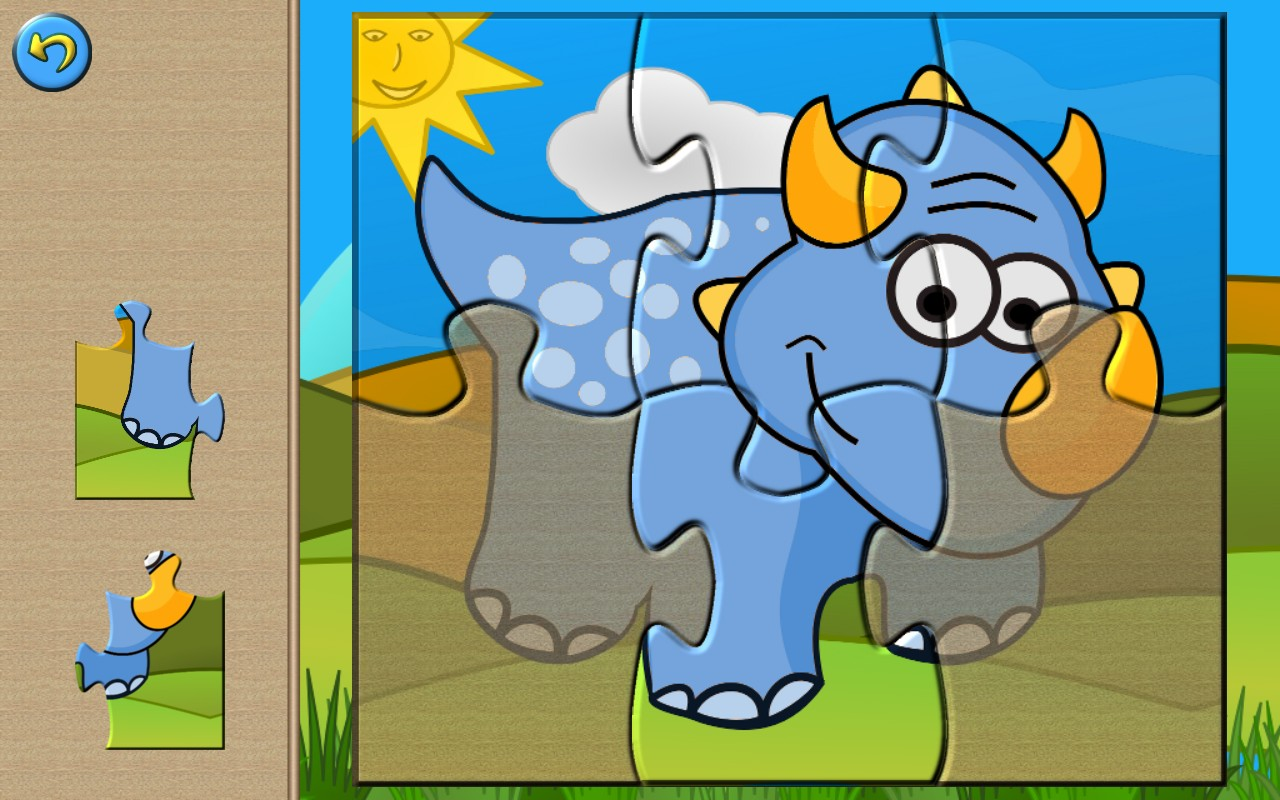
\includegraphics[width=\linewidth]{./Figures/chapter-01/baby-01.jpg}
%		
\includegraphics[width=\linewidth,height=\textheight]{./Figures/chapter-01/baby-02.jpg}
%	\caption{}
\end{figure}
\end{frame}


%%%%%%%%%%%%%%%%%%%%%%%%%%%%%%%%%%%%%%%%%%%%%%%%%%%%%%
\begin{frame}
\frametitle{Transnational DB Use cases}
\begin{figure}[ht]

\centering
%	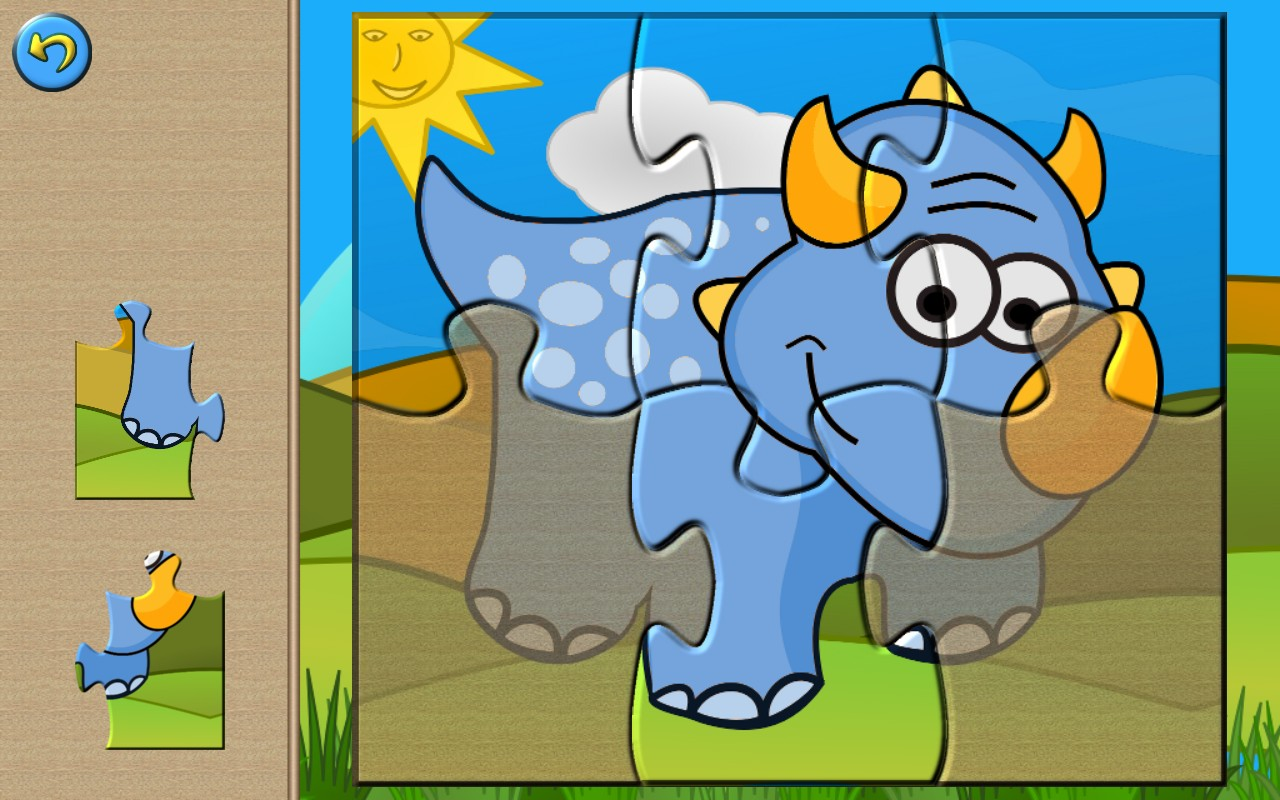
\includegraphics[width=\linewidth]{./Figures/chapter-01/baby-01.jpg}

\includegraphics[width=\linewidth]{./Figures/chapter-01/baby-02.jpg}
%	\caption{}
\end{figure}
\end{frame}


%%%%%%%%%%%%%%%%%%%%%%%%%%%%%%%%%%%%%%%%%%%%%%%%%%%%%%
\begin{frame}
\frametitle{DWH Use cases}
\begin{figure}[ht]

\centering
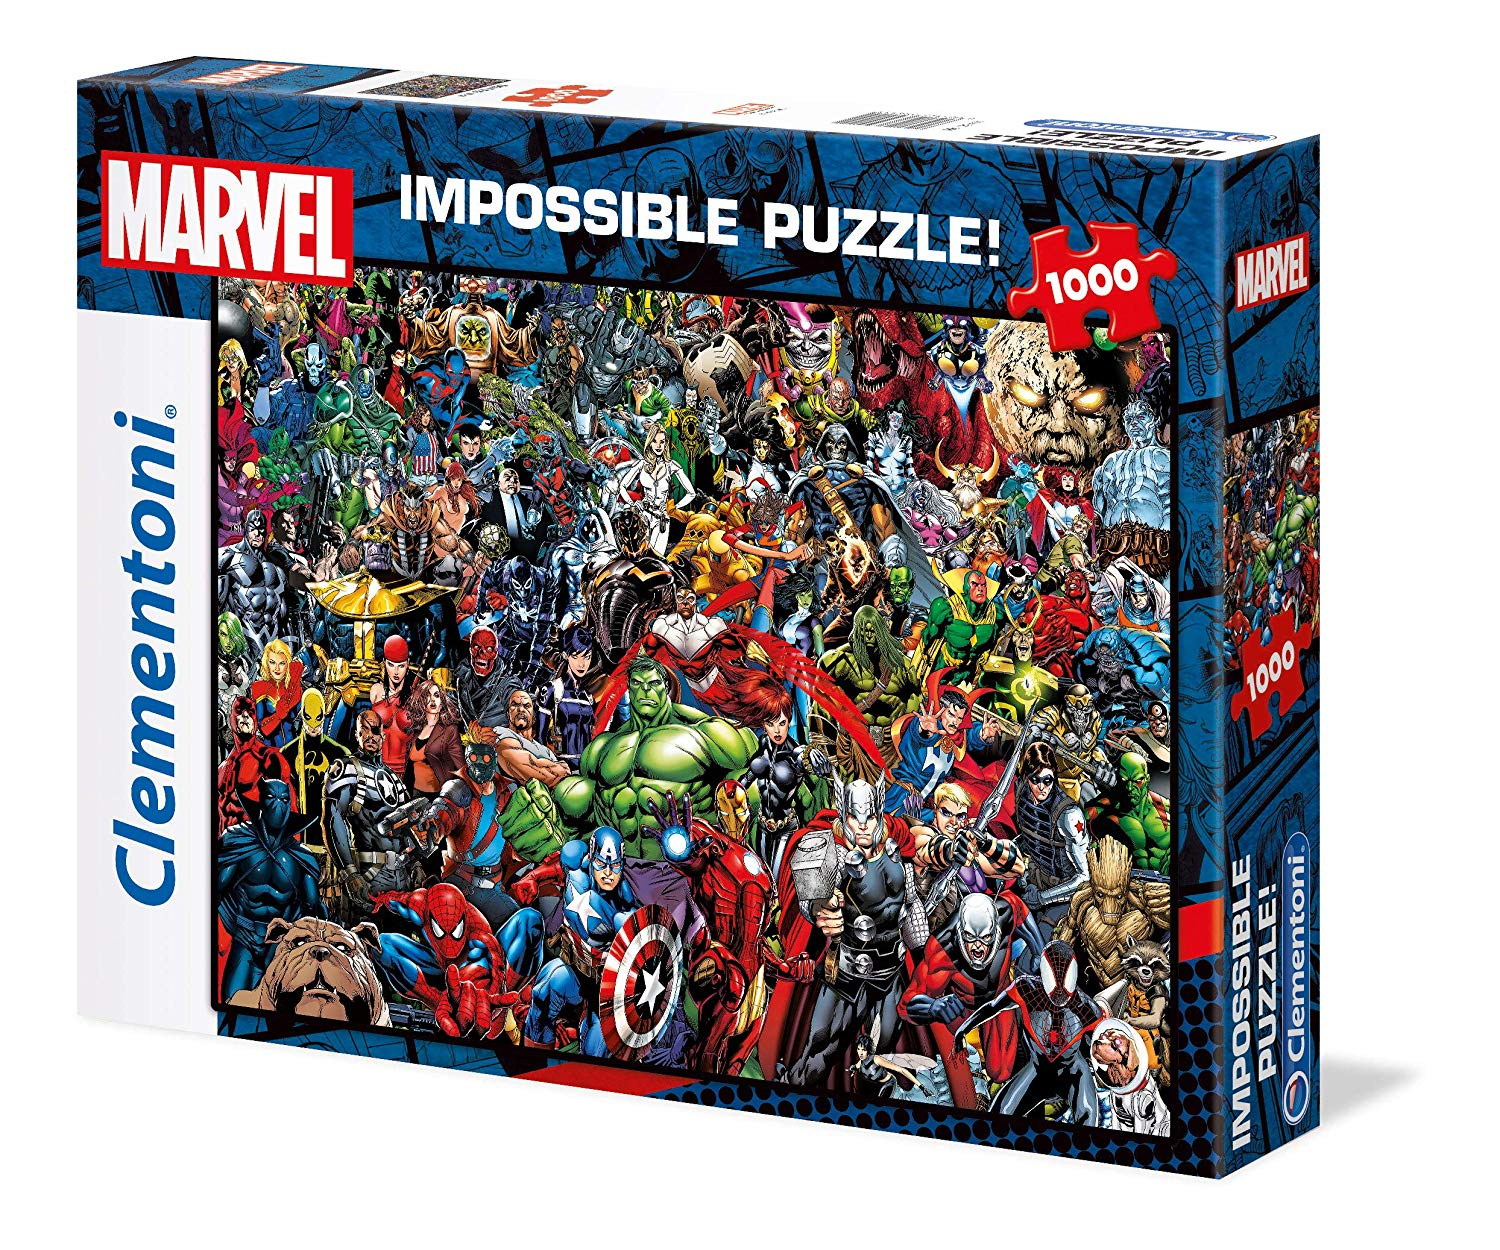
\includegraphics[width=\linewidth,height=.8\textheight]{./Figures/chapter-01/Marvel-03.jpg}
%	\caption{}
\end{figure}
\end{frame}

%%%%%%%%%%%%%%%%%%%%%%%%%%%%%%%%%%%%%%%%%%%%%%%%%%%%%%
\begin{frame}
\frametitle{DWH Use cases}
\begin{figure}[ht]

\centering
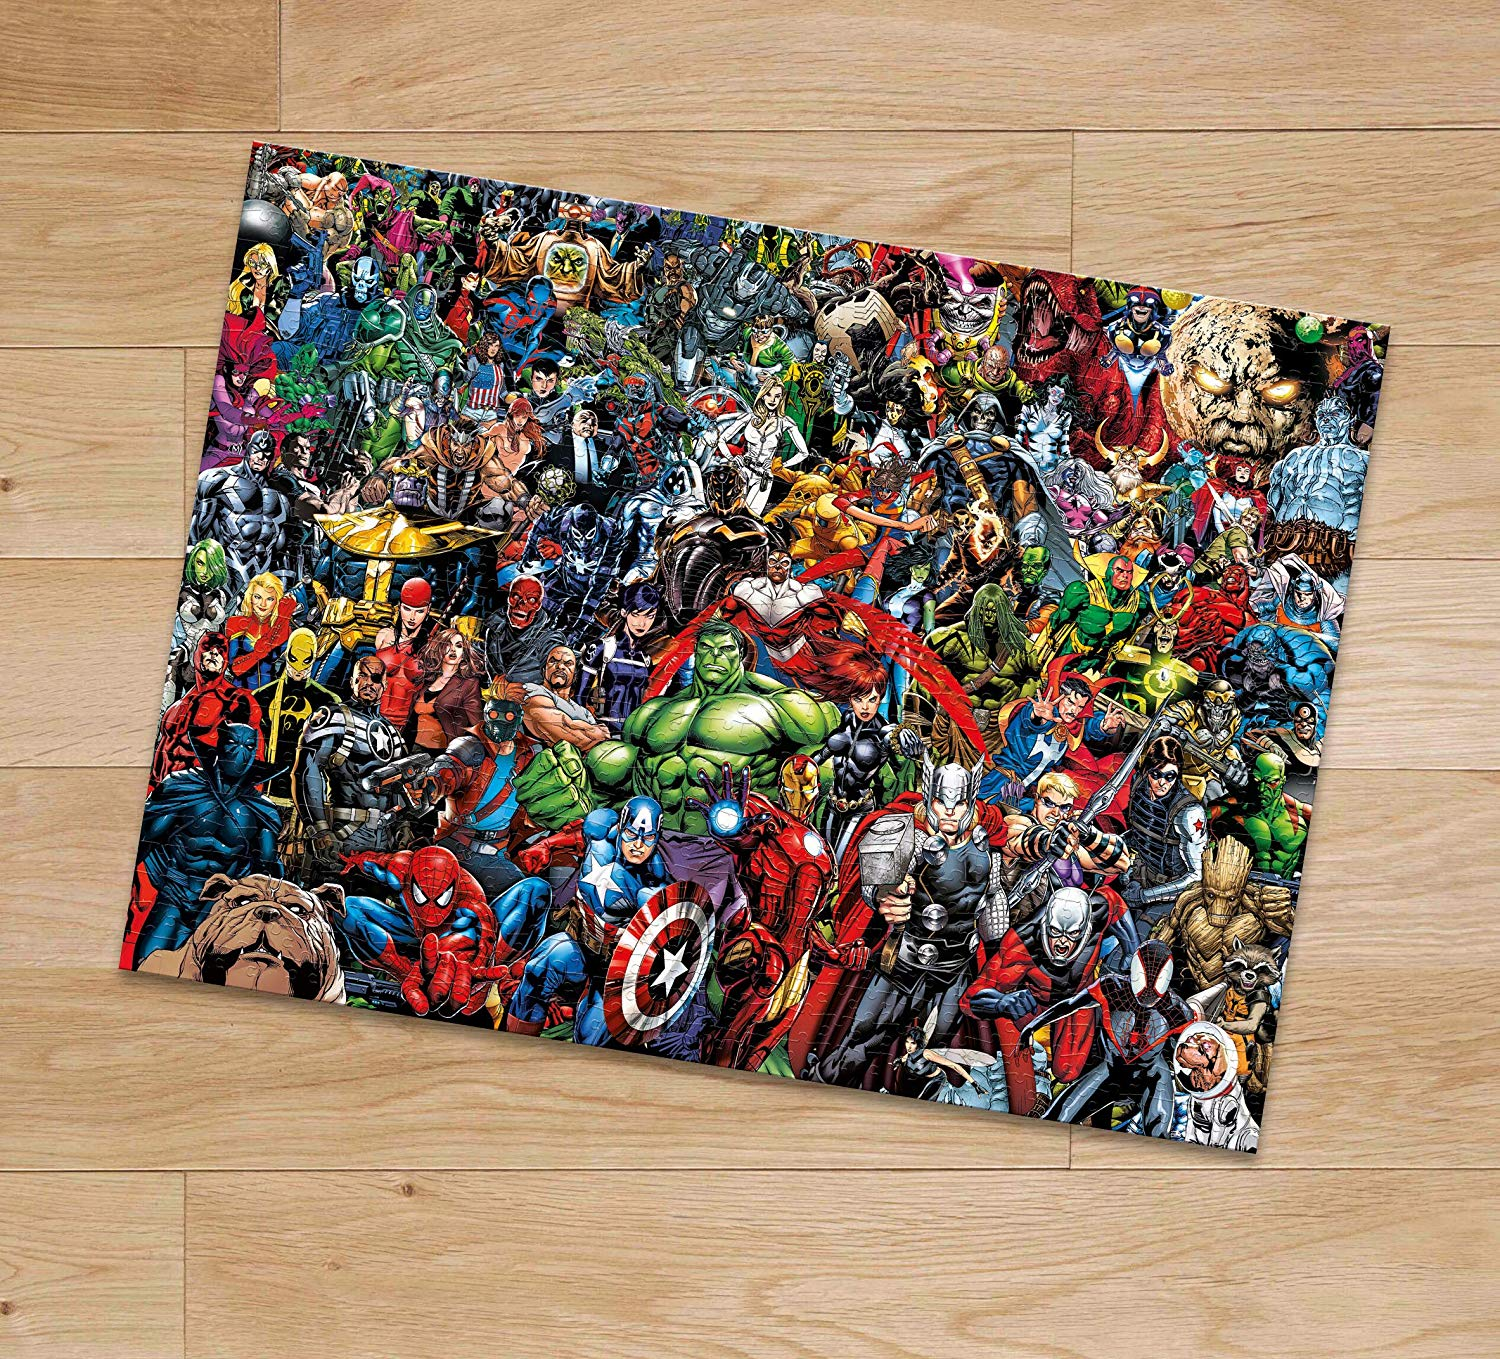
\includegraphics[width=\linewidth,height=.8\textheight]{./Figures/chapter-01/Marvel-02.jpg}
%	\caption{}
\end{figure}
\end{frame}

%%%%%%%%%%%%%%%%%%%%%%%%%%%%%%%%%%%%%%%%%%%%%%%%%%%%%%
\begin{frame}
\frametitle{DWH Use cases}
\begin{figure}[ht]

\centering
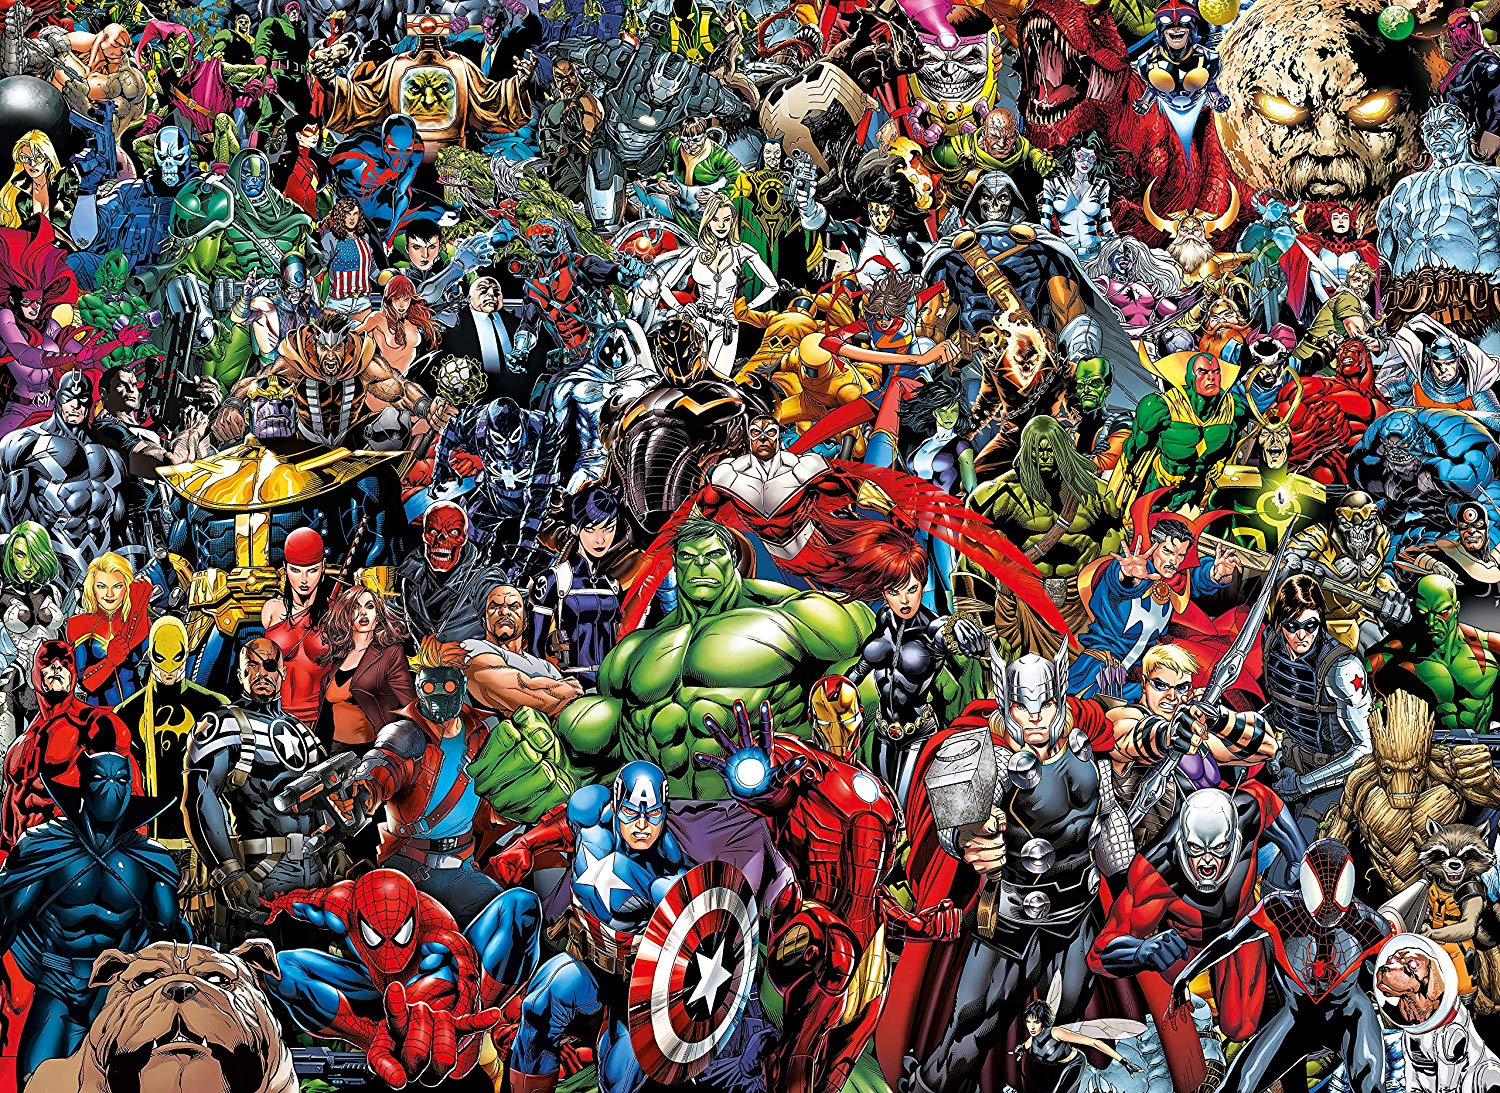
\includegraphics[width=\linewidth,height=.8\textheight]{./Figures/chapter-01/Marvel-01.jpg}
%	\caption{}
\end{figure}
\end{frame}
%%%%%%%%%%%%%%%%%%%%%%%%%%%%%%%%%%%%%%%%%%%%%%%%%%%%%%

\begin{frame}
\frametitle{Use case (Operational DB)}

\begin{itemize}[<+->]

\item A telecommunication company named \textbf{XTec}.
\newline
\item They have lots of systems. One of this systems is a CRM system as example of operational DB.
\begin{itemize}[<+->]

\item The CRM system handles the customer activities with the company including (sales, change in customer plans, and other activities).
\item This system has a backend database (MySQL).
\item CRM team can report their sales and customer activities from their database.
\item Product owner can take a decision based on their system backend reports.

\end{itemize}

\end{itemize}

\end{frame}
%%%%%%%%%%%%%%%%%%%%%%%%%%%%%%%%%%%%%%%%%%%%%%%%%%%%%%

%%%%%%%%%%%%%%%%%%%%%%%%%%%%%%%%%%%%%%%%%%%%%%%%%%%%%%

\begin{frame}
\frametitle{Use case (DWH)}

\begin{itemize}[<+->]

\item What is the need for DWH?		
\begin{itemize}[<+->]
\item This company has other systems for example: billing, charging, signaling.	
\item They need to report information related to the CRM, billing, and signaling source systems in one report.
\item So, they need to ingest (transfer) the data from the source systems to one single database.
\item The decision from the DHW is a \textbf{global and strategical decision.}
\item If the company needs to build a machine learning model which needs data from different sources. They need to load the data from a centralized database rather than read each source alone.
\end{itemize}

\end{itemize}

\end{frame}
%%%%%%%%%%%%%%%%%%%%%%%%%%%%%%%%%%%%%%%%%%%%%%%%%%%%%%


\begin{frame}
\frametitle{Use case (DWH)}
\centering
The Full picture required a DWH. However, we still need the other operational databases for product development perspective.


\end{frame}
%%%%%%%%%%%%%%%%%%%%%%%%%%%%%%%%%%%%%%%%%%%%%%%%%%%%%%

\begin{frame}
\frametitle{Use case (ODS)}
\centering

\begin{itemize}[<+->]
\item Why do we need the ODS?
\item 	How does it fit in our system?
\end{itemize}


\end{frame}
%%%%%%%%%%%%%%%%%%%%%%%%%%%%%%%%%%%%%%%%%%%%%%%%%%%%%%


%%%%%%%%%%%%%%%%%%%%%%%%%%%%%%%%%%%%%%%%%%%%%%%%%%%%%%

\begin{frame}
\frametitle{Use case (ODS)}
\centering
\textbf{XTec} has a call center system which handles the customer inquiries. This system requires the some data related to usage, customer information, billing details to be calculated and accumulated in \textbf{real-time} to be able to give the customer the right answer for his inquires.

\end{frame}
%%%%%%%%%%%%%%%%%%%%%%%%%%%%%%%%%%%%%%%%%%%%%%%%%%%%%%
%%%%%%%%%%%%%%%%%%%%%%%%%%%%%%%%%%%%%%%%%%%%%%%%%%%%%%
\begin{frame}
\frametitle{Use case (ODS)}

	\begin{itemize}[<+->]
		\item So, What is the challenge for this system?
			\begin{itemize}[<+->]		
				\item It needs specific information from different source systems.
				\item It requires to track the source system database changes or update in real-time.
				\item It's functionality is based on the aggregate data not the transactions for example (It needs the total outgoing calls till time or it needs the total charging amounts from prepaid or the available limits from billing if it is postpaid).
			\end{itemize}
	\end{itemize}

\end{frame}
%%%%%%%%%%%%%%%%%%%%%%%%%%%%%%%%%%%%%%%%%%%%%%%%%%%%%%
%%%%%%%%%%%%%%%%%%%%%%%%%%%%%%%%%%%%%%%%%%%%%%%%%%%%%%

\begin{frame}
\frametitle{Use case (ODS)}

	\begin{itemize}[<+->]
		\item ODS is based on change data capture (CDC). This approach used to determine the data change and apply action based on this change.
		\item ODS uses the real-time aggregations to support the online systems from different source systems.
	\end{itemize}
\end{frame}
%%%%%%%%%%%%%%%%%%%%%%%%%%%%%%%%%%%%%%%%%%%%%%%%%%%%%%

\begin{frame}
	\frametitle{DWH Architecture Overview}
	\begin{figure}[ht]
		
		\centering
		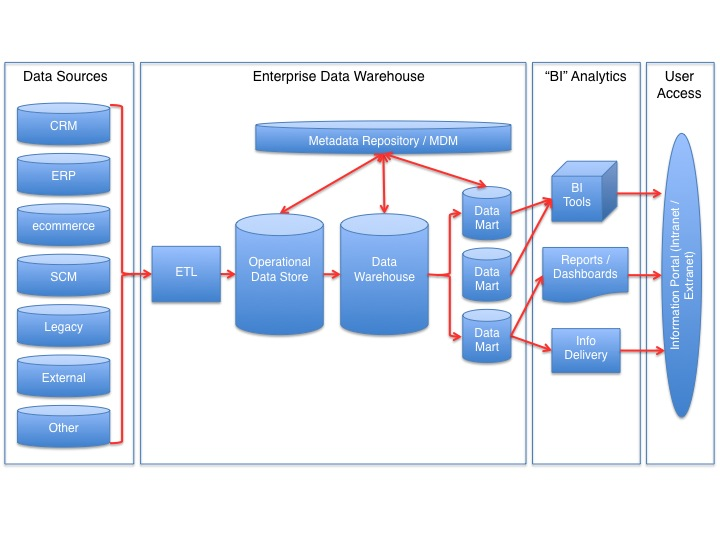
\includegraphics[width=.9\linewidth,height=.8\textheight]{./Figures/chapter-01/Datawarehouse_reference_architecture.jpg}
		%https://commons.wikimedia.org/wiki/File:Datawarehouse_reference_architecture.jpg
		%		
\includegraphics[width=\linewidth,height=\textheight]{./Figures/chapter-01/baby-02.jpg}
			\caption{taken from XXXX}
	\end{figure}
\end{frame}

%%%%%%%%%%%%%%%%%%%%%%%%%%%%%%%%%%%%%%%%%%%%%%%%%%%%%%
\begin{frame}
	\frametitle{Data Abstraction}
	Database systems are made-up of complex data structures. To ease the user interaction with database, the developers hide internal irrelevant details from users. This process of hiding irrelevant details from user is called data abstraction.
	\begin{itemize}[<+->]
		\item There are 3 levels of data abstraction.
		\begin{itemize}[<+->]
			\item Physical level
			\item Logical/ Conceptual level.
			\item View level.
		\end{itemize}
	\end{itemize}		
\end{frame}
%%%%%%%%%%%%%%%%%%%%%%%%%%%%%%%%%%%%%%%%%%%%%%%%%%%%%%
%%%%%%%%%%%%%%%%%%%%%%%%%%%%%%%%%%%%%%%%%%%%%%%%%%%%%%
\begin{frame}
	\frametitle{Data Abstraction}
	\begin{itemize}[<+->]
		\item \textbf{Physical level}: This is the lowest level of data abstraction. It describes how data is actually stored in database. You can get the complex data structure details at this level.
		
		\item \textbf{Logical level}: This is the middle level of 3-level data abstraction architecture. It describes what data is stored in database.
		
		\item \textbf{View level}: Highest level of data abstraction. This level describes the user interaction with database system.
		
	\end{itemize}		
\end{frame}
%%%%%%%%%%%%%%%%%%%%%%%%%%%%%%%%%%%%%%%%%%%%%%%%%%%%%%
\begin{frame}
	\frametitle{Data Abstraction}
	Example: Let’s say we are storing customer information in a customer table. At physical level these records can be described as blocks of storage (bytes, gigabytes, terabytes etc.) in memory. These details are often hidden from the programmers.
	
	At the logical level these records can be described as fields and attributes along with their data types, their relationship among each other can be logically implemented. The programmers generally work at this level because they are aware of such things about database systems.
	
	At view level, user just interact with system with the help of GUI and enter the details at the screen, they are not aware of how the data is stored and what data is stored; such details are hidden from them.
\textbf{	Data Models is the logical level.}
we will discribte the logical level and how can we propsose the external view for the end users.
Regarding the physical level we will not dig dive at this level but for the next chapters we will discuss it in Hadoop, Kafka, Cassandra.
\end{frame}
%%%%%%%%%%%%%%%%%%%%%%%%%%%%%%%%%%%%%%%%%%%%%%%%%%%%%%
%%%%%%%%%%%%%%%%%%%%%%%%%%%%%%%%%%%%%%%%%%%%%%%%%%%%%%
\subsection{Data Models}
\begin{frame}
\frametitle{What is data model?}
Data model is
	\begin{itemize}[<+->]
		\item An abstract model that organizes elements of data.
		\item It describes the objects, entities and data structure properties, semantic, and constraint.
		\item It formalizes the relationship between entities.
		\item It describes how application (report) API data manipulation.
		\item It describes the conceptual design of a business or an application with its flow, logic, semantic information (rules), and how things are done.
		\item It refers to a set of concepts used in defining such as entities, attributes, relations, or tables.
	\end{itemize}
\end{frame}

%%%%%%%%%%%%%%%%%%%%%%%%%%%%%%%%%%%%%%%%%%%%%%%%%%%%%%
\begin{frame}
\frametitle{What is data model?}

\begin{columns}[T] % align columns
	\begin{column}{.45\textwidth}
		Data model is not	
		\begin{itemize}
			\item a science.
			\item a static design for each organization.
			\item a type of database.
			\item a new invention which needs to be done for each project.
		\end{itemize}
		
		\end{column}%
		\hfill%
		\begin{column}{.45\textwidth}
		Data model is		
			\begin{itemize}
				\item an engineering design practices.
				\item a general concepts which lead to build full architecture.
				\item different based on the use case and the database type.
				\item customizable and we can utilize some of ready built architecture. 
				\item implementing using different ways.
				\item affecting the information reporting performance and ways.
			\end{itemize}
		
		\end{column}%
	\end{columns}

\end{frame}
%%%%%%%%%%%%%%%%%%%%%%%%%%%%%%%%%%%%%%%%%%%%%%%%%%%%%%

\begin{frame}
\frametitle{Why does data models are important?}
	\begin{wideitemize}	
		\item Data models are currently affecting software design. 
		\item It decides how engineers will think about the problem they are solving.
	\end{wideitemize}
\end{frame}
%%%%%%%%%%%%%%%%%%%%%%%%%%%%%%%%%%%%%%%%%%%%%%%%%%%%%%
\subsubsection{Data Model Design}
\begin{frame}
\frametitle{Data Model Design vs Implementation}
	\begin{itemize}[<+->]
	\item You need to build a home. So, how do we design this home?
		\begin{itemize}[<+->]
			\item Determine if the home is one level or multi-level and decide man bedrooms and bathrooms for each floor. (User needs)
			\item Hire an architect to put the architecture in more detailed way for example, the size for each room, the distribution of the wireds, where the plumbing fixtures will be placed, etc. (Architecture phase)
			\item Decide the decorations, colors for each room, carpets, etc. 
		\end{itemize}
	\item What do we do for the implementation?
		\begin{itemize}[<+->]
			\item Hire a contractor to build (implement the design) the home. 
			\item This phase will implement the design but it also include some detail related to the actual way to build the tools and the material. (Physical Design)
		\end{itemize}		
	\end{itemize}
\end{frame}
%%%%%%%%%%%%%%%%%%%%%%%%%%%%%%%%%%%%%%%%%%%%%%%%%%%%%%

\begin{frame}
\frametitle{DWH Characteristics}



some details about hot vs cold storage,

\end{frame}

%%%%%%%%%%%%%%%%%%%%%%%%%%%%%%%%%%%%%%%%%%%%%%%%%%%%%%
\begin{frame}

\frametitle{Cold storage vs Hot storage}

some details about hot vs cold storage,

\end{frame}
%%%%%%%%%%%%%%%%%%%%%%%%%%%%%%%%%%%%%%%%%%%%%%%%%%%%%%

\subsubsection{Data Encoding and Formats}
\begin{frame}
\frametitle{\subsecname}
\begin{itemize}[<+->]
\item Any Big Data solution working based distributed systems.
\item What is distributed systems in brief?
\end{itemize}
\end{frame}
%%%%%%%%%%%%%%%%%%%%%%%%%%%%%%%%%%%%%%%%%%%%%%%%%%%%%%%%%%%%%%%%%%%%%%%%%%%

\subsection{Further Readings and Assignment}


%%%%%%%%%%%%%%%%%%%%%%%%%%%%%%%%%%%%%%%%%%%%%%%%%%%%%%%%%%%%%%%%%%%%%%%%%%%
%%% Local Variables:
%%% mode: latex
%%% TeX-master: "../main"
%%% TeX-engine: xetex
%%% End:
